
%(BEGIN_QUESTION)
% Copyright 2007, Tony R. Kuphaldt, released under the Creative Commons Attribution License (v 1.0)
% This means you may do almost anything with this work of mine, so long as you give me proper credit

Her vises sprangresponsen til en prosess med regulatoren i manuell modus. Regn ut prosessforsterkningen ($K$), tidskonstanten ($\tau$) og døtiden ($\theta$).


$$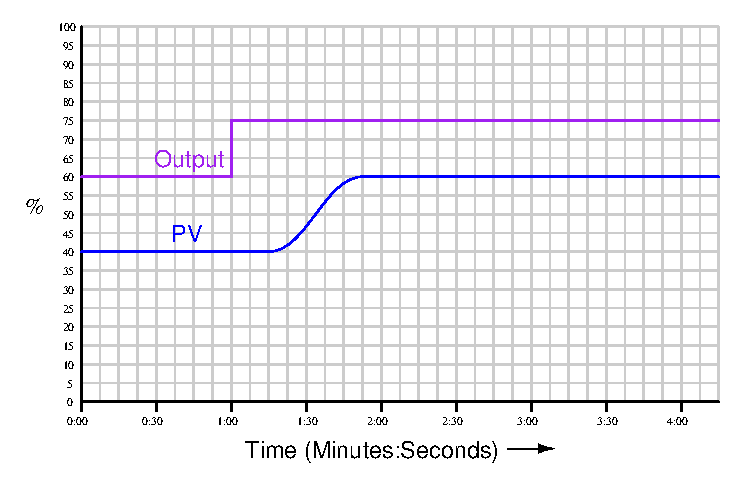
\includegraphics[width=15.5cm]{i01656x01.eps}$$

$K$ = \underbar{\hskip 50pt} \hskip 50pt $\tau$ = \underbar{\hskip 50pt} \hskip 50pt $\theta$ = \underbar{\hskip 50pt}

\vskip 10pt

Anta at vi gjør et mindre sprang i MV på prosessen, f.eks. 35\% istedenfor 15\%, hvilken effekt vil dette ha på $\tau$ og $\Theta$


\vskip 10pt


\underbar{file i01656}
%(END_QUESTION)





%(BEGIN_ANSWER)


%(END_ANSWER)





%(BEGIN_NOTES)

%INDEX% Control, PID tuning: step change (output) revealing process gain
%INDEX% Control, PID tuning: step change (output) revealing process dead time
%INDEX% Control, PID tuning: step change (output) revealing process reaction rate

%(END_NOTES)


